\chapter {Data preprocessing}

\section{Filling missing values}

The main issue is to put a vote on non played matches for each player.
\\
Two approaches have been implemented to achieve this goal, as follow:
\begin{itemize}
\item \textbf{Linear interpolation}: missing values are interpolated using the existing ones; by increasing the cardinality of missing values, this method obviously loses effectiveness but, on the other hand, missing values tend to reflect self trend for each player. (Figure \ref{fig:linear_interpolation})  
\item \textbf{Constant placeholder}: a fixed value is set for each missing vote 
\\
$placeholder = minVote - 1$
\\
No assumption on filled vote confidency can be made since the value is indipendent from player itself. (Figure \ref{fig:placeholder})
\end{itemize}

Chosen a method, all three dataset are modified, and no missing vote is left.

\begin{figure}[H]
  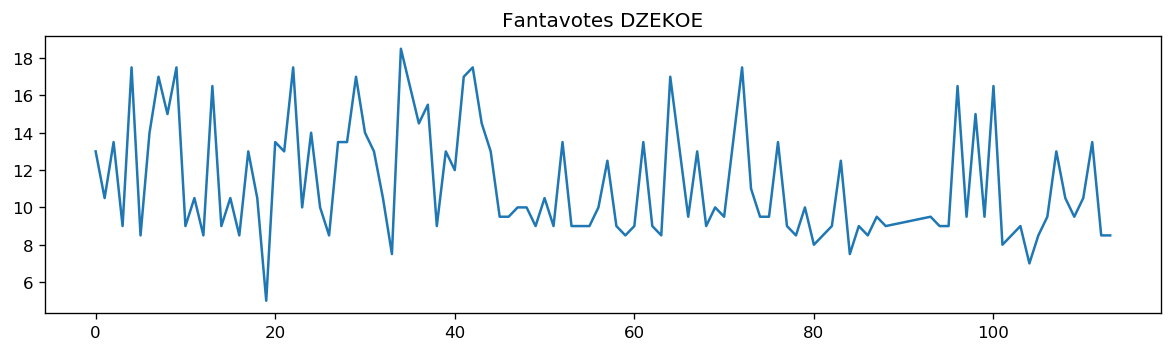
\includegraphics[scale=0.5]{images/dzeko_linear_interpolation_fantavotes.png}
   \centering  
   \caption{\textit{Fantavotes of ''Edin Dzeko'' with \textit{linear interpolation}}}
  \label{fig:linear_interpolation}
\end{figure}

\begin{figure}[H]
  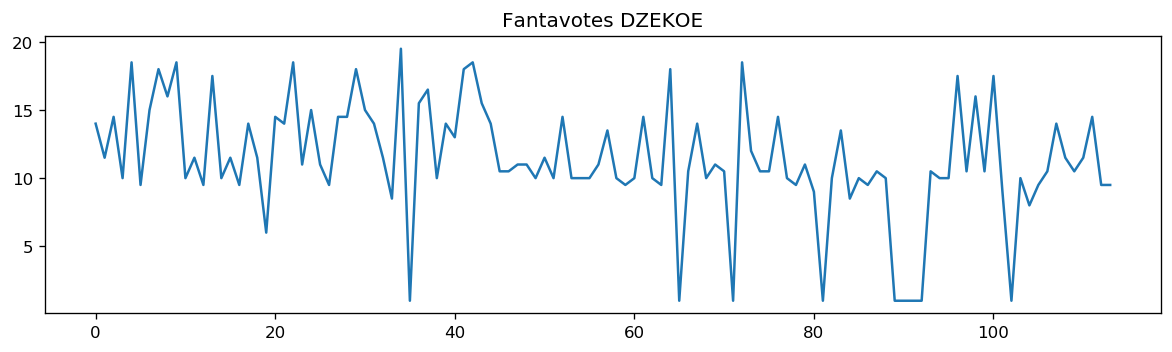
\includegraphics[scale=0.5]{images/dzeko_placeholder_fantavotes.png}
   \centering  
   \caption{\textit{Fantavotes of ''Edin Dzeko'' with \textit{placeholder}}}
  \label{fig:placeholder}
\end{figure}

\section{Translation}
Since votes can be negative we decided to coherently translate them up in order to have all positive values; this was necessary, for example, to eventually apply log transform operations. 

